\chapter{\label{res2}All-optical control of neural circuits across brain regions}

\minitoc

As referenced in the previous section on behaviour, we employed an "all-optical" approach, using light to both record neural activity and experimentally manipulate it, thus driving behaviour. This approach has previously been implemented to study individual brain regions \cite{dalgleish_how_2020, gill_precise_2020, russell_influence_2019, daie_targeted_2021, marshel_cortical_2019}, however here we adapted previous established all-optical procedures to study multiple brain regions, and how activity propagates between them to guide behaviour. 

\section{Localisation of S1 and S2}

To achieve this, we developed a preparation whereby activity in two brain regions (S1 and S2) was recorded simultaneously, while photostimulation was targeted to S1. To read and write neural activity, We expressed the genetically encoded calcium indicator GCaMP6s \cite{chen_ultrasensitive_2013} and the somatically targeted, red-shifted opsin C1V1-Kv2.1 \cite{yizhar_neocortical_2011, chettih_single-neuron_2019} in layer 2/3 across both S1 and S2. A cranial window was implanted to enable optical access to both regions simultaneously. We localised S1 and S2 by performing wide-field calcium imaging during deflection of individual whiskers (Figure \ref{fig:widefield}; methods). We stimulated whisker individually (Figure \ref{fig:widefield}A), recording bulk calcium activity, and thus localising the somatotopic representation of the whisker pad indicative of S1 and S2 (Figure \ref{fig:widefield}B-E). Mice were only trained on behavioural tasks if they expressed opsin in S1 and calcium indicator in S1 and S2. In subsequent all-optical experiments, a field of view was selected which spanned multiple barrels of the a, b and c row both in S1 and S2 (Figure \ref{fig:widefield}B).

\begin{figure}[h]
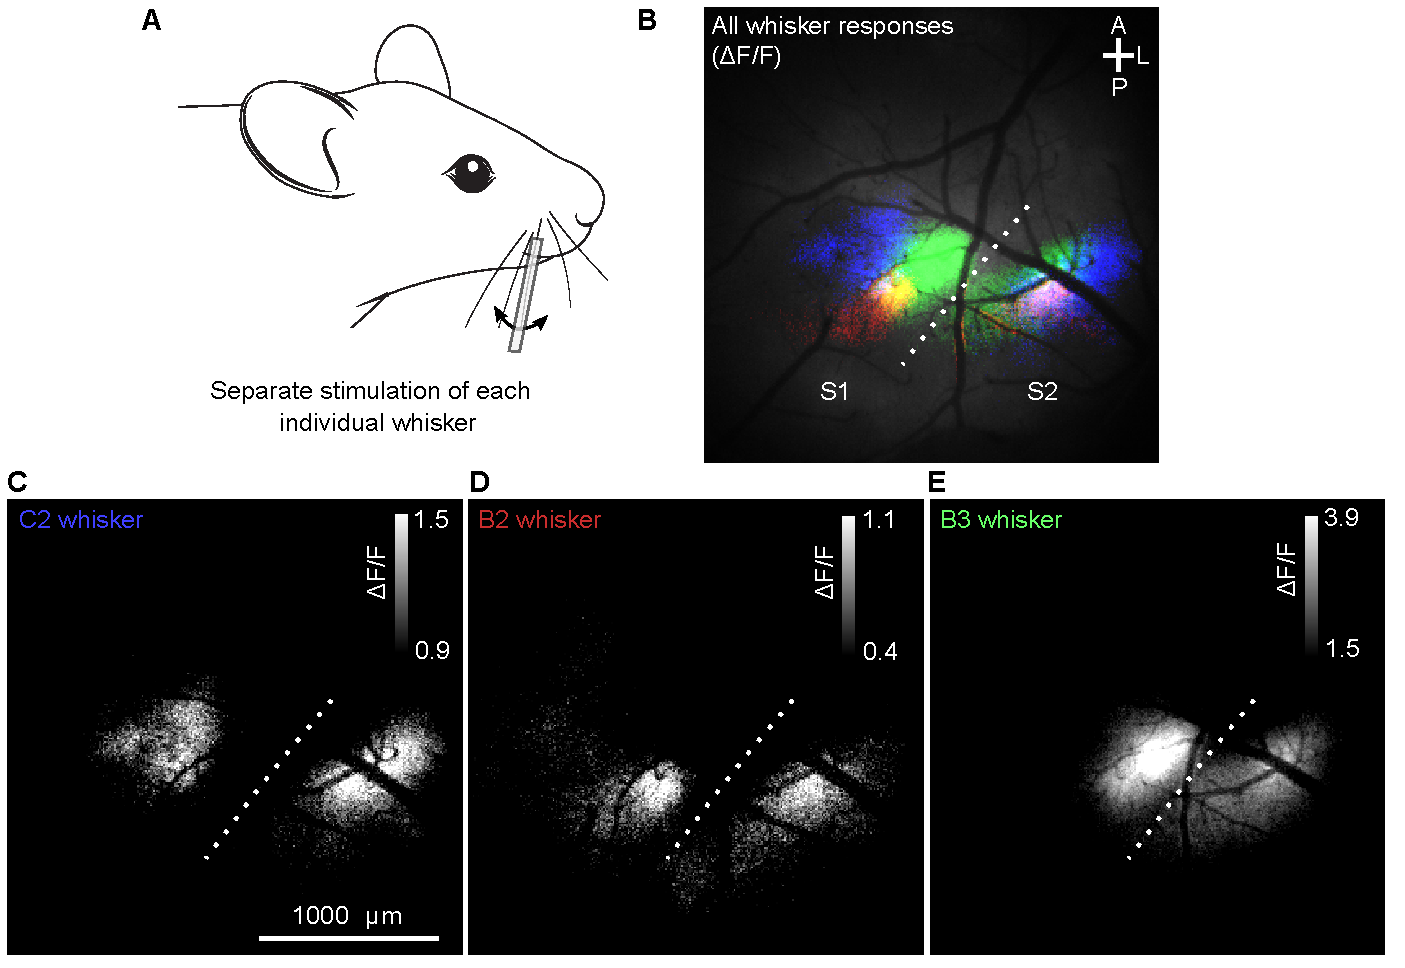
\includegraphics[scale=0.62]{figures/widefield-localisation.pdf}
\caption[\textbf{Widefield localisation of S1 and S2}]{
\textbf{Widefield localisation of S1 and S2}. \textbf{(A)} Individual whiskers of head-fixed mice were threaded into a capillary and deflected to elicit a neural response in the corresponding barrel. \textbf{(B)} Composite image showing a map of the barrel fields spanning S1 and S2 for an example mouse. \textbf{(C)} Trial averaged $\Delta$F/F responses from bulk widefield calcium imaging, across S1 and S2, following stimulation of the C2 whisker. \textbf{(D)} As C but for the B2 whisker. \textbf{(E)} As C but for the B3 whisker.
} 
\label{fig:widefield}
\end{figure}

\section{Simultaneous two-photon calcium imaging and photostimulation}

To read and write neural activity \textit{in vivo} across brain regions in a behaving animal, we employed a two-photon microscope, based on previous designs \cite{packer_simultaneous_2015}, adapted to perform two-photon calcium imaging of neural activity across a large field of view (1.35 mm diameter), while performing two-photon photostimulation of S1 neurons. As outlined in the previous section, mice expressing a calcium indicator and an opsin were head-fixed and the objective lens of the microscope was placed directly over a cranial window. 

Calcium imaging was performed with a resonant scanning systems (Figure \ref{fig:all-optical}A), scanning at 30 Hz, to excite and image the genetically encoded calcium indicator GCaMP6s \cite{chen_behaviour-dependent_2013} (Figure \ref{fig:2-photon-behaviour}A). Spikes inferred from the slow ‘ultrasensitive’ variants of GCaMP have been shown to have correlations of >0.85 with ground truth spike trains \cite{friedrich_fast_2017}.

To photo-activate groups of cells simultaneously, we used a microscope with
a spatial light modulator (SLM) incorporated into the beam path of a laser capable of
two-photon excitation (Figure \ref{fig:all-optical}A). The SLM contains a reflective liquid crystal layer which acts as a two-dimensional diffraction grating, and thus can be combined with  holography to target multiple beamlets of light to arbitrary, user-defined points in space. This is demonstrated in Figure \ref{fig:all-optical}B in which fluorescence generated from 54 simultaneously generated beamlets was imaged on a wide-field camera.

The spatial resolution of an optical system is generally quantified using the point-spread function (PSF). In relation to imaging, this defines the smallest object that can be visualised, as the recorded image results from the convolution of the actual object and the PSF. The resolution of a two-photon imaging system is conventionally defined as the full width half max (FWHM) of the PSF and is usually degraded most in the axial dimension \cite{shaw_point-spread_1991}. The PSF can be recorded by imaging a sub-resolution florescence source. The axial resolution for the resonant imaging system is shown in Figure \ref{fig:all-optical}C left, generated by taking a "z-stack" to generate a 3-dimensional image of the sub-resolution source from two-dimensional images taken a different focal depths. The PSF profile was then fit with a Gaussian function from the axial fluorescence intensity profile of the source, yielding a FWHM of 2.99 $\mu$m. This process can be repeated with the photostimulation beam, reflected off the SLM, to generate an image of a PSF describing the profile of the photostimulation beamlet on the sample, thus quantifying the resolution of the photostimulation system (Figure \ref{fig:all-optical}C right, FWHM = 19.8 $\mu$m). These two PSFs demonstrate that theoretically our microscope is able to read and write activity in individual neurons.

A proof-of-principle example of how the two-photon calcium imaging and optogenetics can be used to read and write neural activity is shown in Figures \ref{fig:all-optical}D and E. Figure \ref{fig:all-optical}D shows calcium activity, recorded through fluorescence imaging of GCaMP6s, a surrogate for spikes \cite{chen_ultrasensitive_2013, huang_relationship_2021, grienberger_imaging_2012, packer_simultaneous_2015, stosiek_vivo_2003}. Figure \ref{fig:all-optical}E demonstrates how neural activity can be injected into individual neurons expressing opsin, without driving spikes in neighbouring opsin-expressing neurons. Only the  cell targeted with two-photon photostimulation exhibits a clear increase in fluorescence locked  temporally to the stimulus onset.

\begin{figure}[!h]
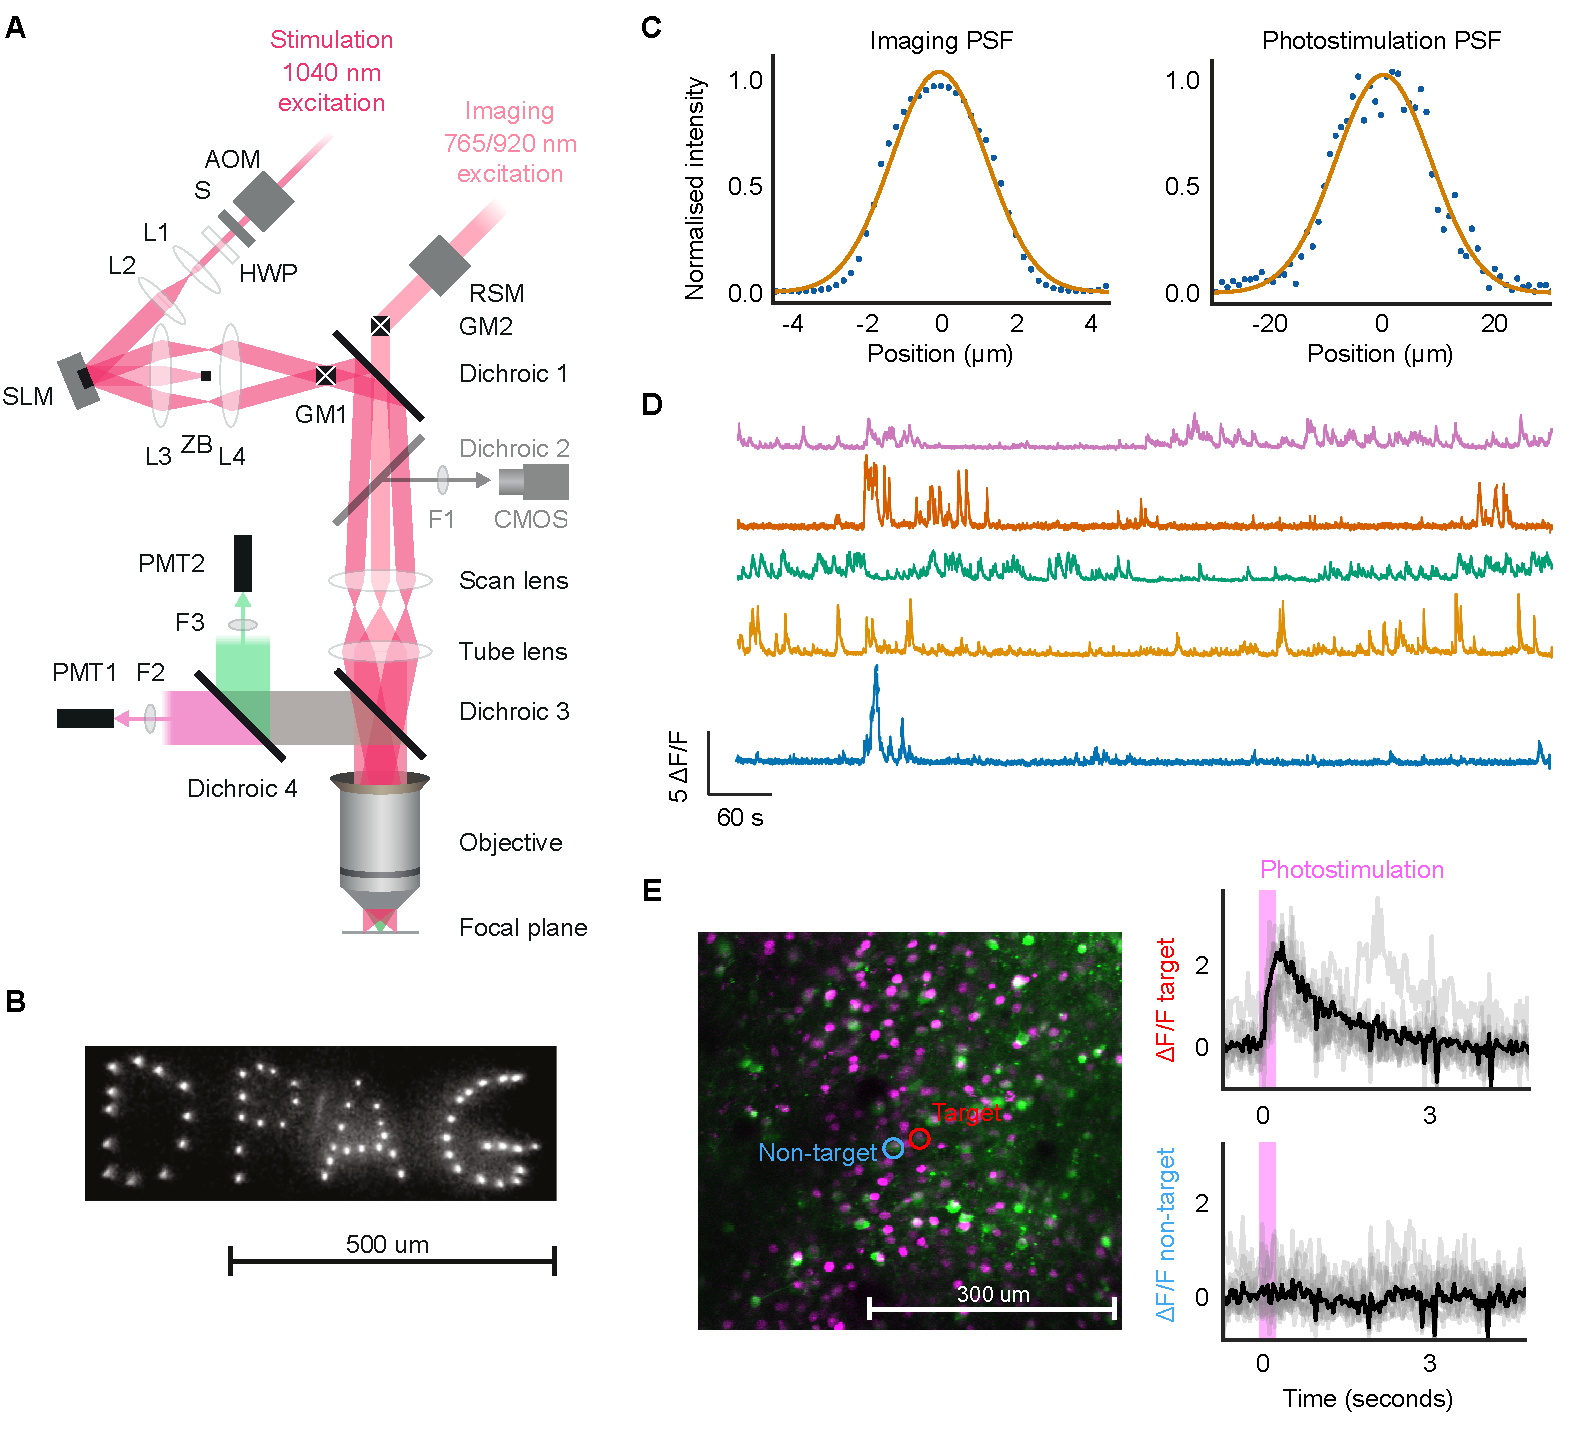
\includegraphics[scale=0.567]{figures/2p_imaging+photostim.pdf}
\caption[\textbf{Two-photon calcium imaging and photostimulation}]{
\textbf{Two-photon calcium imaging and photostimulation. (A)} Layout of the all-optical beam path. AOM, acousto-optic modulator; S, shutter; HWP, half-wave plate; L1-4, lenses; SLM, spatial light modulator; ZB, zero order block; GM1,GM2, galvanometers; RSM, resonant scanning module; F1-3, filters; PMT1, PMT2, photomultiplier tubes. Adapted from \cite{packer_simultaneous_2015}. \textbf{(B)} Beamlets generated by splitting the photostimulation beam with the SLM. For display purposes beamlets were imaged on a fluorescent plastic slide using a widefield camera (DPAG = department of physiology, anatomy and genetics). \textbf{(C)} \textit{Left}: Axial PSF of the resonant imaging system (FWHM = 2.99 um). \textit{Right}: Axial PSF of the photo-stimulation system (FWHM
= 19.8 um). \textbf{(D)} Example calcium traces from 5 neurons imaged at 30 Hz. Traces were smoothed for display with a running mean of 3 frames. \textbf{(E)} \textit{Left}: Example field of view of a mouse. expressing the calcium indicator GCaMP6s (green) and the opsin ST-ChroME (magenta) (used only for this calibration experiment). The cell targeted for two-photon holographic photostimulation is highlighted in blue. \textit{Right}: Fluorescence traces resulting from 10 trials of targeted photostimulation. Individual trials are shown in grey and the mean response across all trials is shown in black. 
} 
\label{fig:all-optical}
\end{figure}

While these proof of principal experiments prove that we can photostimulate and record from individual neurons, the behavioural experiment requires that we photostimulate groups of multiple S1 neurons, varying on a trial by trial basis, while imaging across S1 and S2. The principles behind this are outlined in figure \ref{fig:s1s2}. Mice expressing the calcium indictor GCaMP6s \cite{chen_ultrasensitive_2013} and the red-shifted soma-targetted opsin C1V1-kv2.1 \cite{yizhar_neocortical_2011, chettih_single-neuron_2019} were headfixed under the objective of the beam path outlined in figure \ref{fig:all-optical}. 

A field of view was selected which spanned multiple barrels of the a, b and c row both in S1 and S2 which we could image with two-photon calcium imaging with single-cell resolution (Figure \ref{fig:s1s2}B,C). Before the behavioural experiment, we photostimulated all opsin-expressing neurons in multiple small groups, to find cells responsive to photostimulation, with neurons within a 350 μm diameter stimulated simultaneously. Each group of neurons was photostimulated for 250 ms, with 5 ms between the stimulation of each group. Trial averaged, excitatory responses to this "pre-behaviour" photostimulation can be visualised as a stimulus triggered average image (see methods) in which responses were apparent in neurons proximal to the photostimulation beam (“targets”, defined as cells within 15 µm of the center of the beam) (Figure \ref{fig:all-optical}C; methods).

An demonstrative example of how multiple groups of neurons can be targeted in quick succession is shown in figure \ref{fig:s1s2}D. Phase masks are loaded onto the SLM, with a 5 ms inter-mask-interval, resulting in multiple beamlets of light targeted to individual cell soma. As shown in the STA images (methods) from the neural response generated by each of these masks, only cells directly under the photostimulation targets are activated by light. 

As discussed in the previous section, and methods, during behavioural training we targeted between 5 and 150 photoresponsive neurons on each go trial. Groups of between 5 and 50 neurons could be targeted simultaneously with a single phase mask. The cells comprising the groups were chosen randomly with replacement on a trial by trial basis. However our system does not have the photostimulation beam power or spatial range to stimulate 150 cells simultaneously. Hence this was achieved by stimulating 3 groups of 50 neurons, resulting in a total stimulation length of 750 ms. The trial-averaged responses of targeted and non-targeted cells, both in S1 and S2, during behaviour is shown for a single session in figure \ref{fig:s1s2}. A clear excitatory response is only observed, when averaging across trials, in targeted neurons. As the identity of targeted cells was varied trial to trial, the cells averaged to form the traces was not the same on every trial.

\begin{figure}[h]
\includegraphics[scale=0.54]{figures/multiarea_ao.pdf}
\caption[\textbf{All-optical interrogation across brain regions}]{
\textbf{All-optical interrogation across brain regions (A)} Schematic of experimental setup. Left: viral strategy for expression of GCaMP6s and C1V1-KV2.1-mScarlet in S1 and S2.  Right: mice with a cranial window installed over S1 and S2 were headfixed under a two-photon microscope. A lick spout was placed within reach of the tongue, through which the animal reported perception of photostimulation by licking and received a water reward. \textbf{(B)} Example widefield calcium imaging field of view used to localise S1 and S2 by whisker stimulation. \textbf{(C)} Example two-photon calcium imaging field of view with photostimulation targets. The intensity of each pixel is proportional to the change in fluorescence intensity post-photostimulation compared to pre-photostimulation; bright pixels indicate a photostimulation-induced increase in calcium activity. Pixels are color-coded based on whether they were photostimulated simultaneously. Non-targeted cells, including those in S2 are not visible when averaging across a single stimulation group.
\textbf{(D)} Sequential photostimulation. An
automated protocol was used to target groups of cells for simultaneous stimulation. Groups
were stimulated for 250 ms with a 5 ms inter-group-interval. 10 trials of stimulation were
performed. \textit{Top}: Phase masks loaded onto the SLM to generate targets. \textit{Bottom}: STA images (methods). The pixel intensity of the images shows the change in $\Delta$F/F compared to baseline, averaged across trials, in a period of 1 second immediately following photostimulation of the targets (yellow circles). \textbf{(E)} Example activity responses to photostimulation in a single behavioural session. Blue shows the response to photostimulation of cells directly targeted with light, averaged across cells and across trials. Orange and green show the response of cells not directly targeted in S1 and S2 respectively. Only trials in which photostimulation was delivered were included and data were baselined to the pre-stimulus mean on a cell-wise and trial-wise basis before averaging. Data are blanked while the photostimulation laser was on (pink bar) as this causes a large artifact unrelated to neural activity.
} 
\label{fig:s1s2}
\end{figure}

In sum, this chapter demonstrates that I, alongside my colleagues, developed methodologies that allowed, all-optical techniques to be applied across multiple brain regions. This tool can then be combined with the behavioural paradigm outlined in the previous section to study neural activity, causal in behaviour as it propagates between brain regions.
